%
% The MIT License (MIT)
%
% Copyright (c) 2016 Paul Batty
%
% Permission is hereby granted, free of charge, to any person obtaining a copy
% of this software and associated documentation files (the "Software"), to deal
% in the Software without restriction, including without limitation the rights
% to use, copy, modify, merge, publish, distribute, sublicense, and/or sell
% copies of the Software, and to permit persons to whom the Software is
% furnished to do so, subject to the following conditions:
%
% The above copyright notice and this permission notice shall be included in
% all copies or substantial portions of the Software.
%
% THE SOFTWARE IS PROVIDED "AS IS", WITHOUT WARRANTY OF ANY KIND, EXPRESS OR
% IMPLIED, INCLUDING BUT NOT LIMITED TO THE WARRANTIES OF MERCHANTABILITY,
% FITNESS FOR A PARTICULAR PURPOSE AND NONINFRINGEMENT. IN NO EVENT SHALL THE
% AUTHORS OR COPYRIGHT HOLDERS BE LIABLE FOR ANY CLAIM, DAMAGES OR OTHER
% LIABILITY, WHETHER IN AN ACTION OF CONTRACT, TORT OR OTHERWISE, ARISING FROM,
% OUT OF OR IN CONNECTION WITH THE SOFTWARE OR THE USE OR OTHER DEALINGS IN
% THE SOFTWARE.
%

\section{Design}
\label{sec:design}

Having looked at SQLite and the current tools. This chapter will cover the requirements set out for the tool, the features and a high level overview of the architectural design.  Then going into more depth looking at each module that makes up the application. Finishing off looking at how the user interface could look.

\subsection{Requirements}
\label{subsec:requirements}

In the previous chapter this paper showed that there is a lack of tools available that allow an insight into SQLite and how it works. The exception to this was the SQLite fragmentation tool, that did show the file format though not the over arching structure. It also had some severe limitations as as to the types of databases that it would work with. 
\\\\
In addition to this SQLite currently provides no way to log changes performed to the database outside of the currently running program. This is implemented by SQLite itself, to get around this triggers and other such convoluted systems have to be used.
\\\\
It also showed that the file system is put together, constructing a large B-Tree structure. As just mentioned there is no way to view this structure without using a hex editor, and manually following the links.
\\\\
Lastly, most of the SQLite tools are font end user interfaces for SQLite databases. While this is useful for working with SQLite database they provide no way to debug or see what is going on. 
\\\\
In order to address the issues listed above, throughout the remaining sections this paper will design, implement and test a front end user interface tool, that can solve the current situation.
\\\\
The tool itself must be reliable and support the majority of features in the current version of SQLite at the time of writing this paper. It must also not modify the database file in any way to preserve the database, and the data it contains, excluding parts of the application that are specifically designed to. Lastly, the tool must be cross platform and intractable through a user interface. 

\subsection{Features}
\label{subsec:Features}

As just mentioned, there are a lot of issues surrounding the current situation with SQLite tools. The tool this paper will design and implement contains five main features, on top of a single base feature.
\\\\
The central feature is the visualiser. The visualiser allows the visualisation of the broken down page structure and hierarchy of the SQLite database file. Viewing the file broken into pages, and how they connect to each other in the B-Tree structure. On top of this clicking or otherwise interacting with a node to see more information about. Such as data, page number and pointers.
\\\\
In addition to the visualiser, there is will be a metadata tab that will present the header information in the database. Alongside other statistics that come from parsing the database. Such as number of tables, primary keys and version numbers.
\\\\
The base feature allows real time updating of this data when any command from any system modifies the database in some way shape or form. The live updating will allow stepping through the time line of updates that have occurred while the application is running. Lastly, it can be paused to inspect a certain state / place in time. 
\\\\
Whenever a update occurs, all changes that happened are recorded inside a log, and a "snapshot" of the database is taken. This snapshot is then presented to the user, through the visualiser, metadata and log tabs. Creating the time line that can then be browsed. 
\\\\
Apart from just showing you data, you can also execute SQL commands onto the database, through the SQL executor. And view the schema and tables currently inside the database. 
\\\\
Finally, the tool will come with a friendly user interface, through which the user can interact with each of the features. Each feature above aim to address the issues mentioned at the start of this chapter.

\subsection{High level Overview}
\label{subsec:high_level_overview}

From the start I wanted to build a system, that was modular, self-contained and adaptable. In order to accomplish this I decide to use a MVC (Model-View-Controller) architecture in order to separate the interface from the data. This means the view will make requests to the controller, who will then in turn contact the model for information, then sending the information backwards to be presented by the view. The idea being that the view could be switched or adjusted at any time without breaking the application. an example of MVC can be seen below in figure~\ref{fig:mvc}.

\begin{figure}[H]
	\centering
	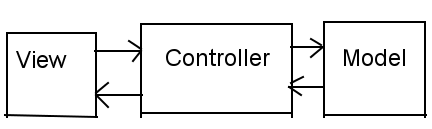
\includegraphics[scale=0.5]{images/mvc.png}
	\caption{MVC architecture}
	\label{fig:mvc}
\end{figure}

With this in mind the bulk of the work is performed inside the model. However, like any project, along the way I ran into some problems and so had to adjust my design. Figure~\ref{fig:design_old} shows the original design.

\begin{figure}[H]
	\centering
	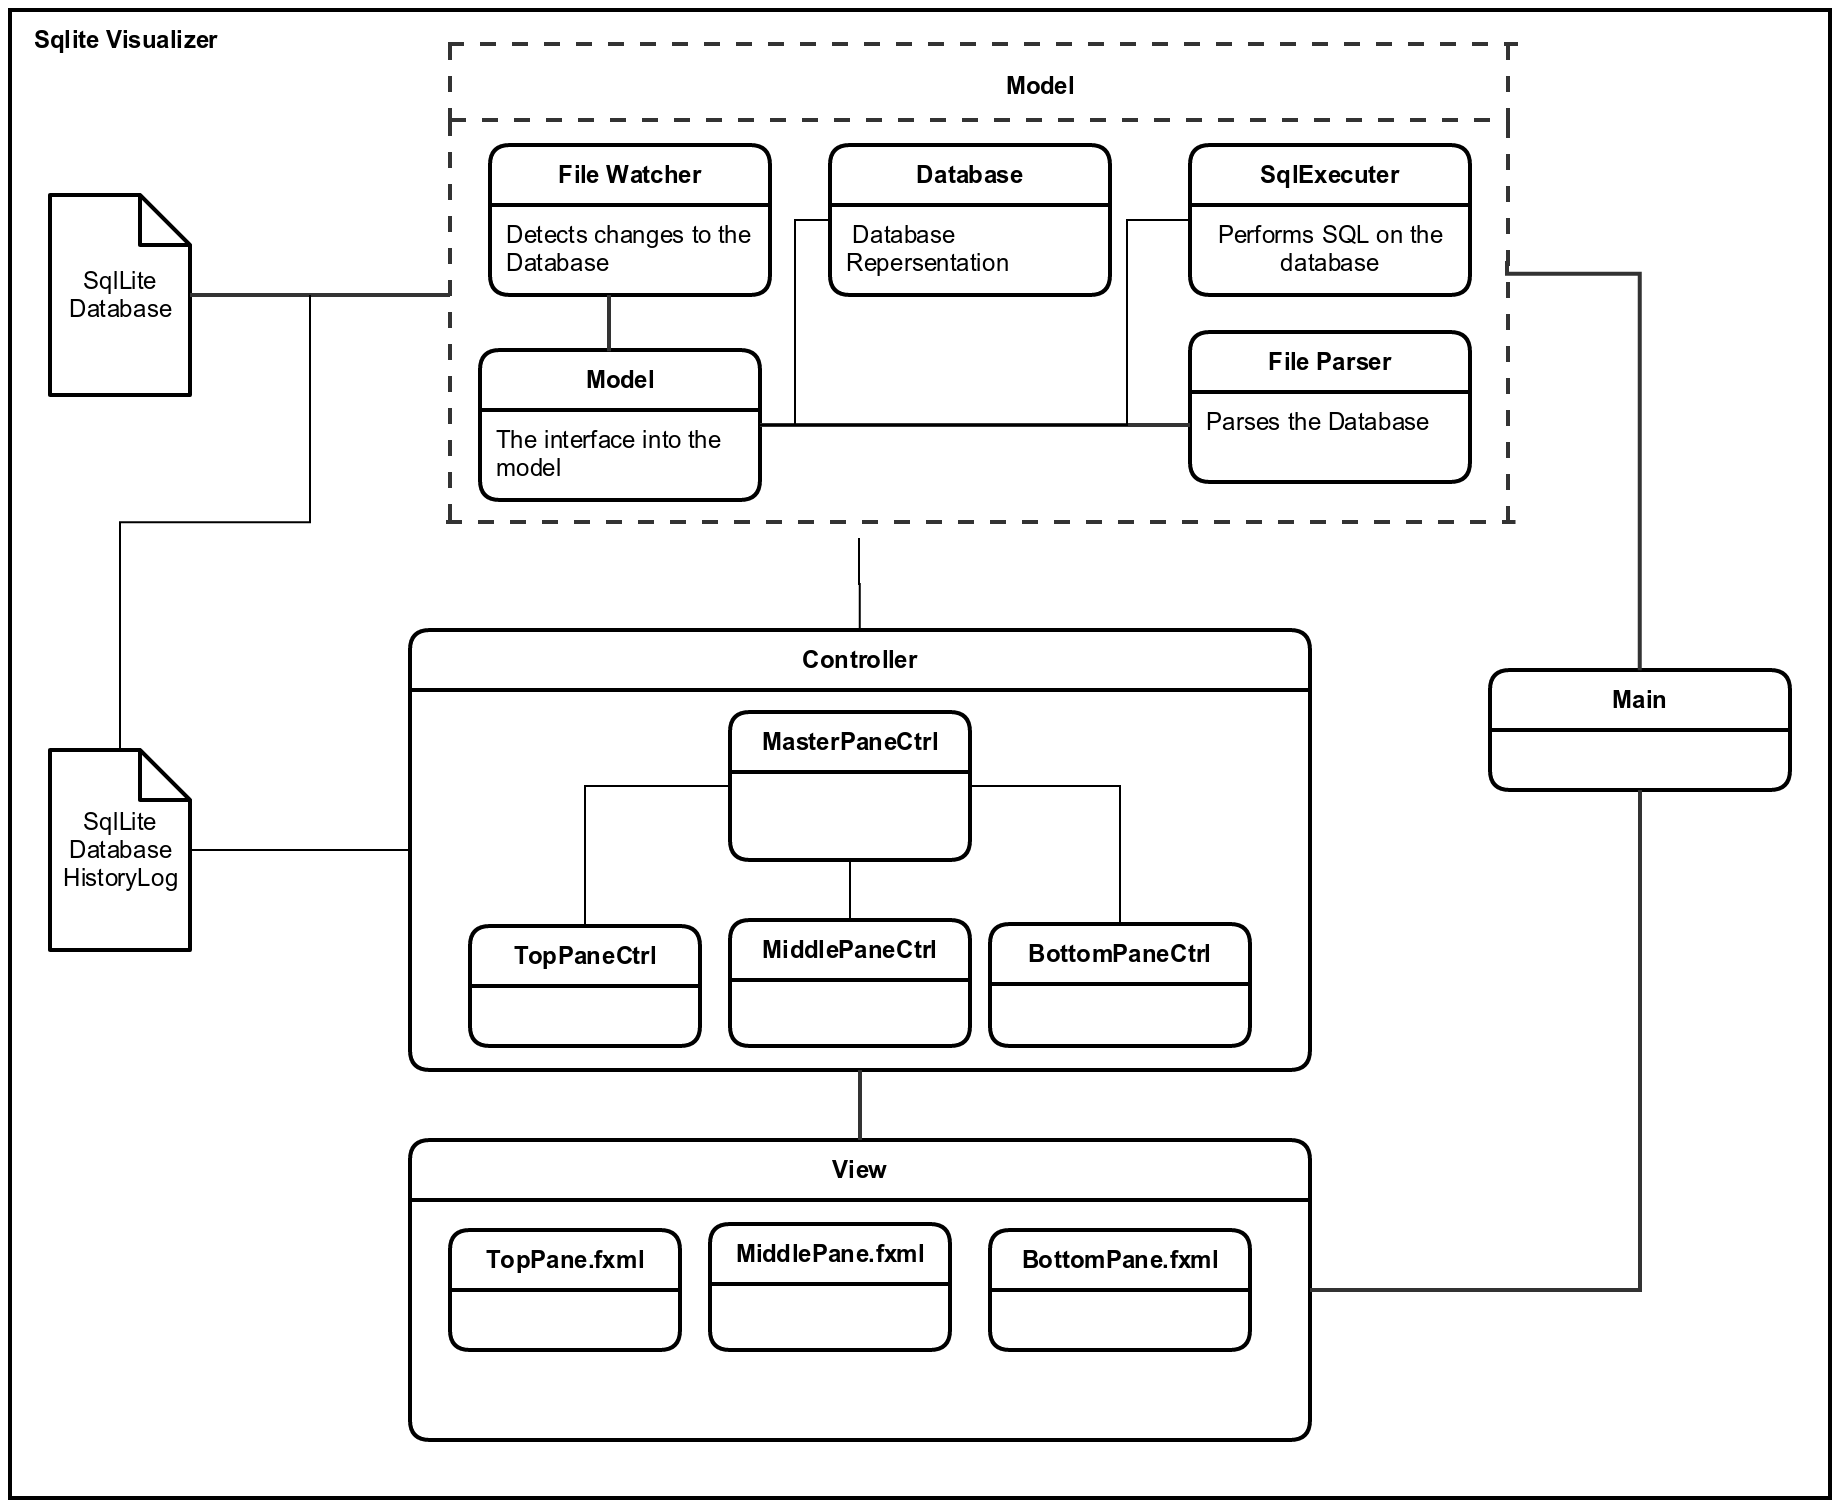
\includegraphics[scale=0.2]{images/system_diagram_old.png}
	\caption{Original system diagram}
	\label{fig:design_old}
\end{figure}

The Model was going to run in its own thread so it could control, manage and prepare the data as it came in. This meant the view could request it when it wanted. The model was also made up of five modules. With the logging  stored into an external file, for the view to read when it wanted. In addition to this the controllers follow a hierarchical structure, with a master controller, controlling access to the model. However, this design proved unusable and thus changed into the following seen in figure~\ref{fig:design_new}. 

\begin{figure}[H]
	\centering
	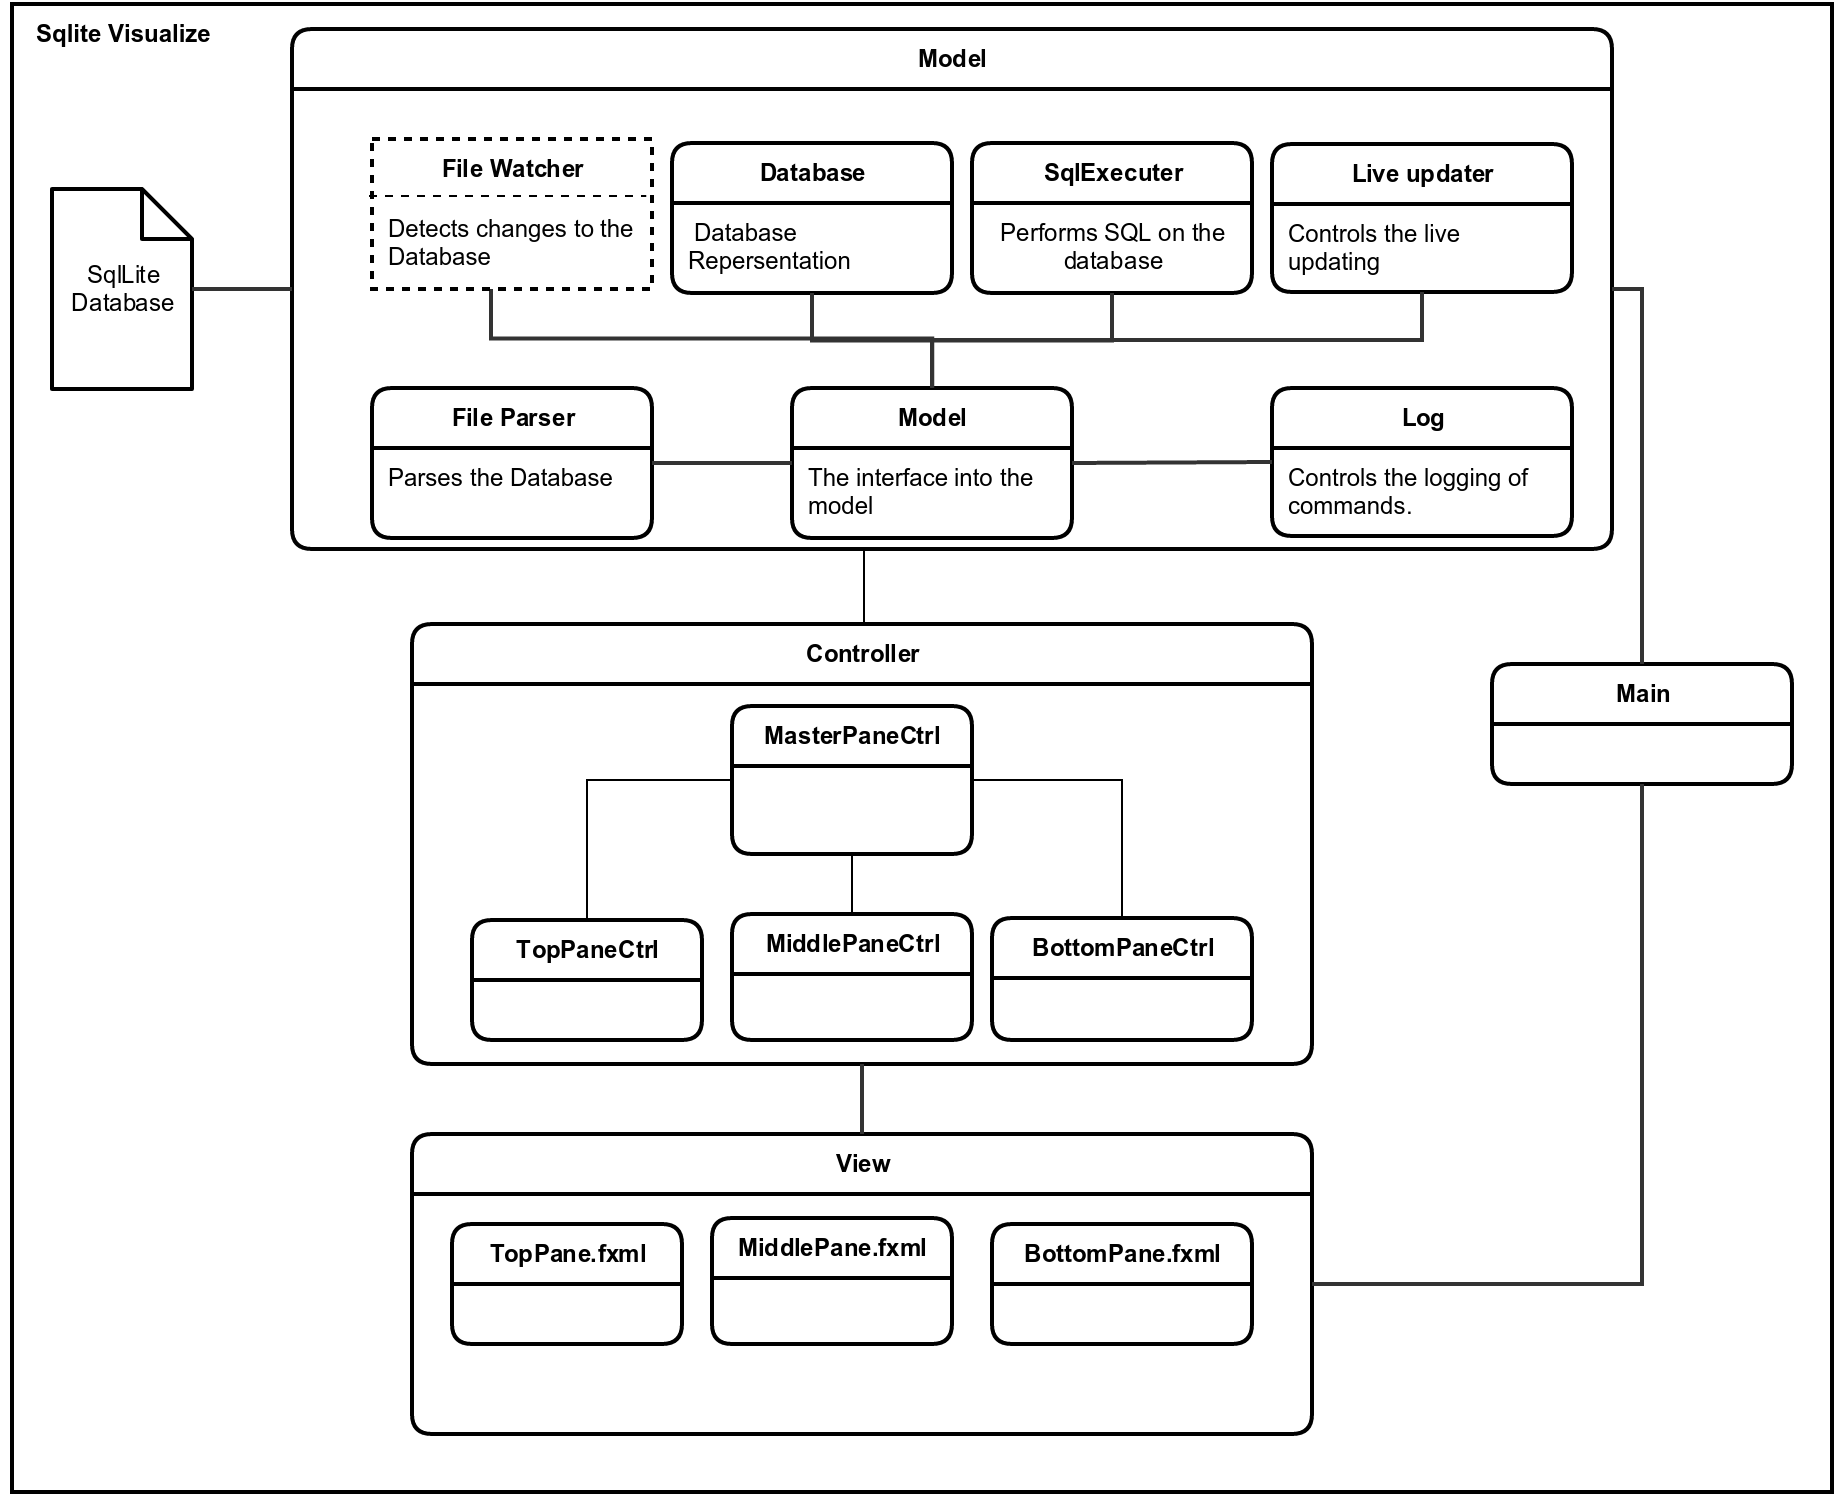
\includegraphics[scale=0.2]{images/system_diagram_new.png}
	\caption{Final system diagram}
	\label{fig:design_new}
\end{figure}

Most of the changes are seen within the Model, with the addition of two new modules. And rather then running the whole thing inside a new thread only the file watcher is. On top of this the command logging is no longer written out to file. The final change is the reduction in the amount of controllers. I will go over each of the modules in the next part.

\subsection{Module Overview}
\label{subsec:module_overview}

\subsubsection{The Main}
\label{subsubsec:main}

The main module represents the staring point of the application, it serves no other purpose other then to correctly initialise the view, model and controllers.

\subsubsection{The View}
\label{subsubsec:the_view}

The view, consists of three parts, the top, middle and right side. The middle section can also be split in half when needed to view two different panes at the same time. In addition to this the top and right sides do not change through the running of the application. The middle section however, changes depending on what is being viewed.

\subsubsection{The Controller}
\label{subsubsec:the_controller}

The controller is made up of two parts, the master controller, and the pane controller. The pane controller is changed depending on what is being viewed. Respectively to the views middle pane. The master controller however stays through the running of the program and coordinates what is being shown. Both of them communicate to the model to collect updates, and interact with the data.

\subsubsection{The Model}
\label{subsubsec:the_model}

The model is the most complicated section and is made up of seven modules. The model itself acts as a repository design with all the modules connecting and interacting though a shared object the model interface.
\\\\
The first module, marked as 'model' represents the model interface. In which all communication, with sub modules, from the controllers will go through. It is also the only class to have direct access to all sub modules, as i tried to keep them as modular and independent as possible. In addition to this, it provides a small amount of functionality for setting up, closing and opening the database. Since every module will require something from this action.
\\\\
The Database, is the in program mapping of the SQLite database file. The database is made up of two parts, the data objects, and the interface into the data objects. The data objects are the mapping of the SQLite database. Containing the B-Tree system, and the data. The interface provides access control to the data objects, allowing the program move along the database time line.
\\\\
The file watcher, runs in a continuous loop, inside its own thread, utilising the observer pattern. The observer patten allows any class to register to it, and will revive a signal when an event occurs. In this case it would be the updating of the database file. When a change is detected, a signal will be sent out over the observers, alerting them to the change. Although, if they did not tune in to the observer, The program would not receive  database updates.
\\\\
The File parser, parses any given valid database file. Converting it into the database object.
\\\\
The log, takes any two database objects and records the changes between them.
\\\\
The live updater, acts like a master controller for the modules, apart from the SQL executor, file watcher and model interface. It controls the program flow when a change is detected, and as such is registered to the file watchers observer. When a change is detected, the first thing it does is contact the file parser for the updated database object, then sends it off to the log, to record changes, before storing it in the database module and incrementing the current position on the time line.
\\\\
The SQL executor, controls the SQL connections, and executes SQL commands onto the database.

\subsection{The User interface}
\label{subsec:high_user_interface}

The user interface is designed to be simplistic and easy to use and familiar to new users. The basic format is a menu bar at the top,  with icons underneath. Just below them is a selection of tabs corresponding to the different views, that the application can take. Down the right hand side, however will be another static section representing the SQl executer. This can be seen below in figure~\ref{fig:design_user_iterface}.

\begin{figure}[H]
	\centering
	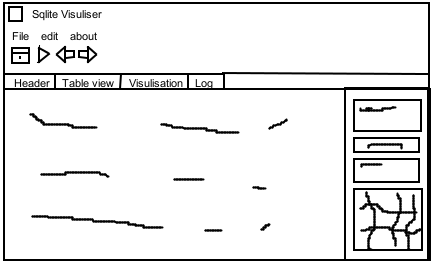
\includegraphics[scale=0.7]{images/ui_design.png}
	\caption{User interface design.}
	\label{fig:design_user_iterface}
\end{figure}

Originally the SQl executor was going to have its own tab. But it worked out better along side the content as you can then view what the commands are doing to the database, when they are ran. Or have the information as a reference when typing up commands, Below figure~\ref{fig:db_browser_screen} shows the SQL executer User interface design.

\begin{figure}[H]
	\centering
	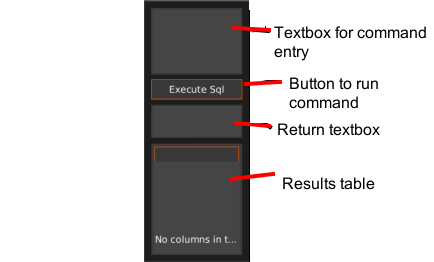
\includegraphics[scale=0.7]{images/ui_sqlexe_design.png}
	\caption{SQL executor design.}
	\label{fig:design_user_iterface}
\end{figure}

The user will type commands into the top text box, and then press the button to run the command. After the command is ran a message will be displayed in the return text box. And any returned data will be presented in the results table.
\\\\
The base live updater is controlled via the icons and drop down menus with the four other features having their own tab. The metadata tab, is designed to have different panes, split up in to data relevance, each showcasing the different values. For example one pane will show the size, another the version numbers and so on. This can be seen below in figure~\ref{fig:des_ui_meta}. 

\begin{figure}[H]
	\centering
	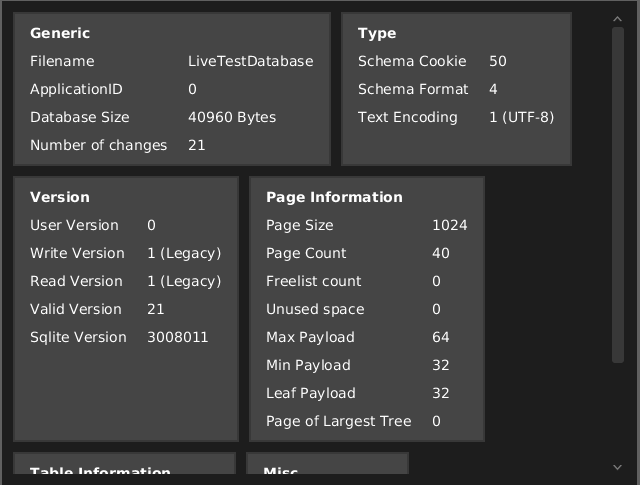
\includegraphics[scale=0.32]{images/ui_meatadata.png}
	\caption{Metadata interface design.}
	\label{fig:des_ui_meta}
\end{figure}

The other feature that is closely tied to this information is the visualiser. The visualiser is made up of two parts, the left hand side where the data will be shown, and the central section showing the visualisation. The visualisation will display the file B-Tree as it is inside the file, with the pages represented as nodes. Then when a node is selected the data will be shown inside the data pane. This can be seen below in figure~\ref{fig:des_ui_vis}.

\begin{figure}[H]
	\centering
	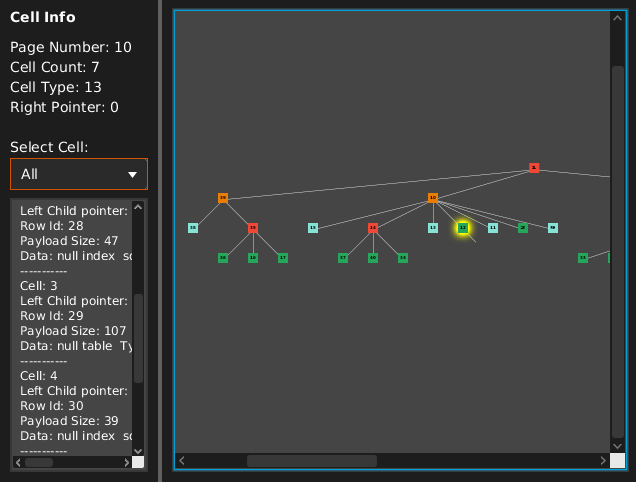
\includegraphics[scale=0.32]{images/ui_visuliser.png}
	\caption{Visualiser interface design.}
	\label{fig:des_ui_vis}
\end{figure}

In the above figure, the glowing node tells the user that this node was updated in the last update. Along side this a log entry is created. The log tab much like the metadata tab will be made up off small panes, titled with the date, and the collapsible content. The content will store what changed in that update this can be seen in figure~\ref{fig:des_ui_log}

\begin{figure}[H]
	\centering
	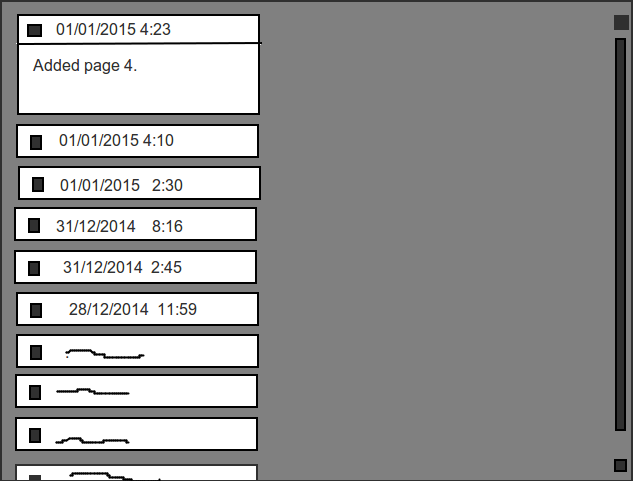
\includegraphics[scale=0.32]{images/ui_log.png}
	\caption{Log interface design.}
	\label{fig:des_ui_log}
\end{figure}

The idea behind the folding panels,  is to allow users to hide information that they do not need. As such if there is a large change it would not be filling the screen. The last feature and tab is the table and schema view. This, much like the visualiser uses two sections. The left, to display the list of tables and the schema. With the centre displaying the table data. This can be seen in figure~\ref{fig:des_ui_table}. 

\begin{figure}[H]
	\centering
	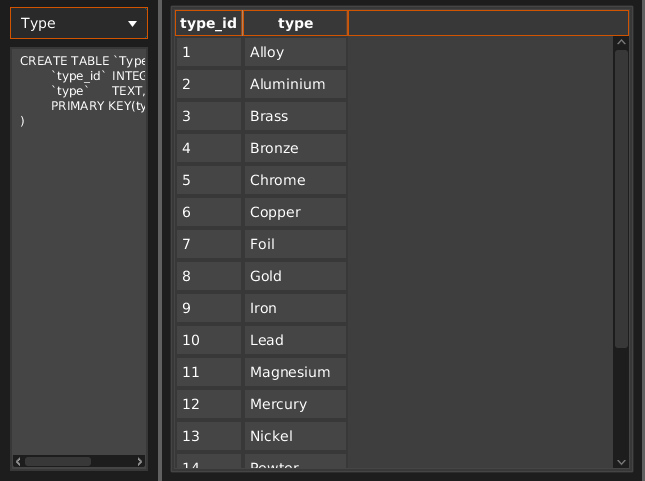
\includegraphics[scale=0.32]{images/ui_table.png}
	\caption{Table interface design.}
	\label{fig:des_ui_table}
\end{figure}
